\clearpage
\section{维修站里的碎石和金属}
从维修站出生点看过去，右侧油桶下方有一大片砂石。最初地上已经有一张记录石面朝向的法线图，画面却像蒙了一层细沙。下图来自两次正式运行的游戏。人物、天空、灯光、曝光和镜头沿用关卡设置，截取的都是游戏第 12 帧。

\begin{center}
\panelimage{.48\linewidth}{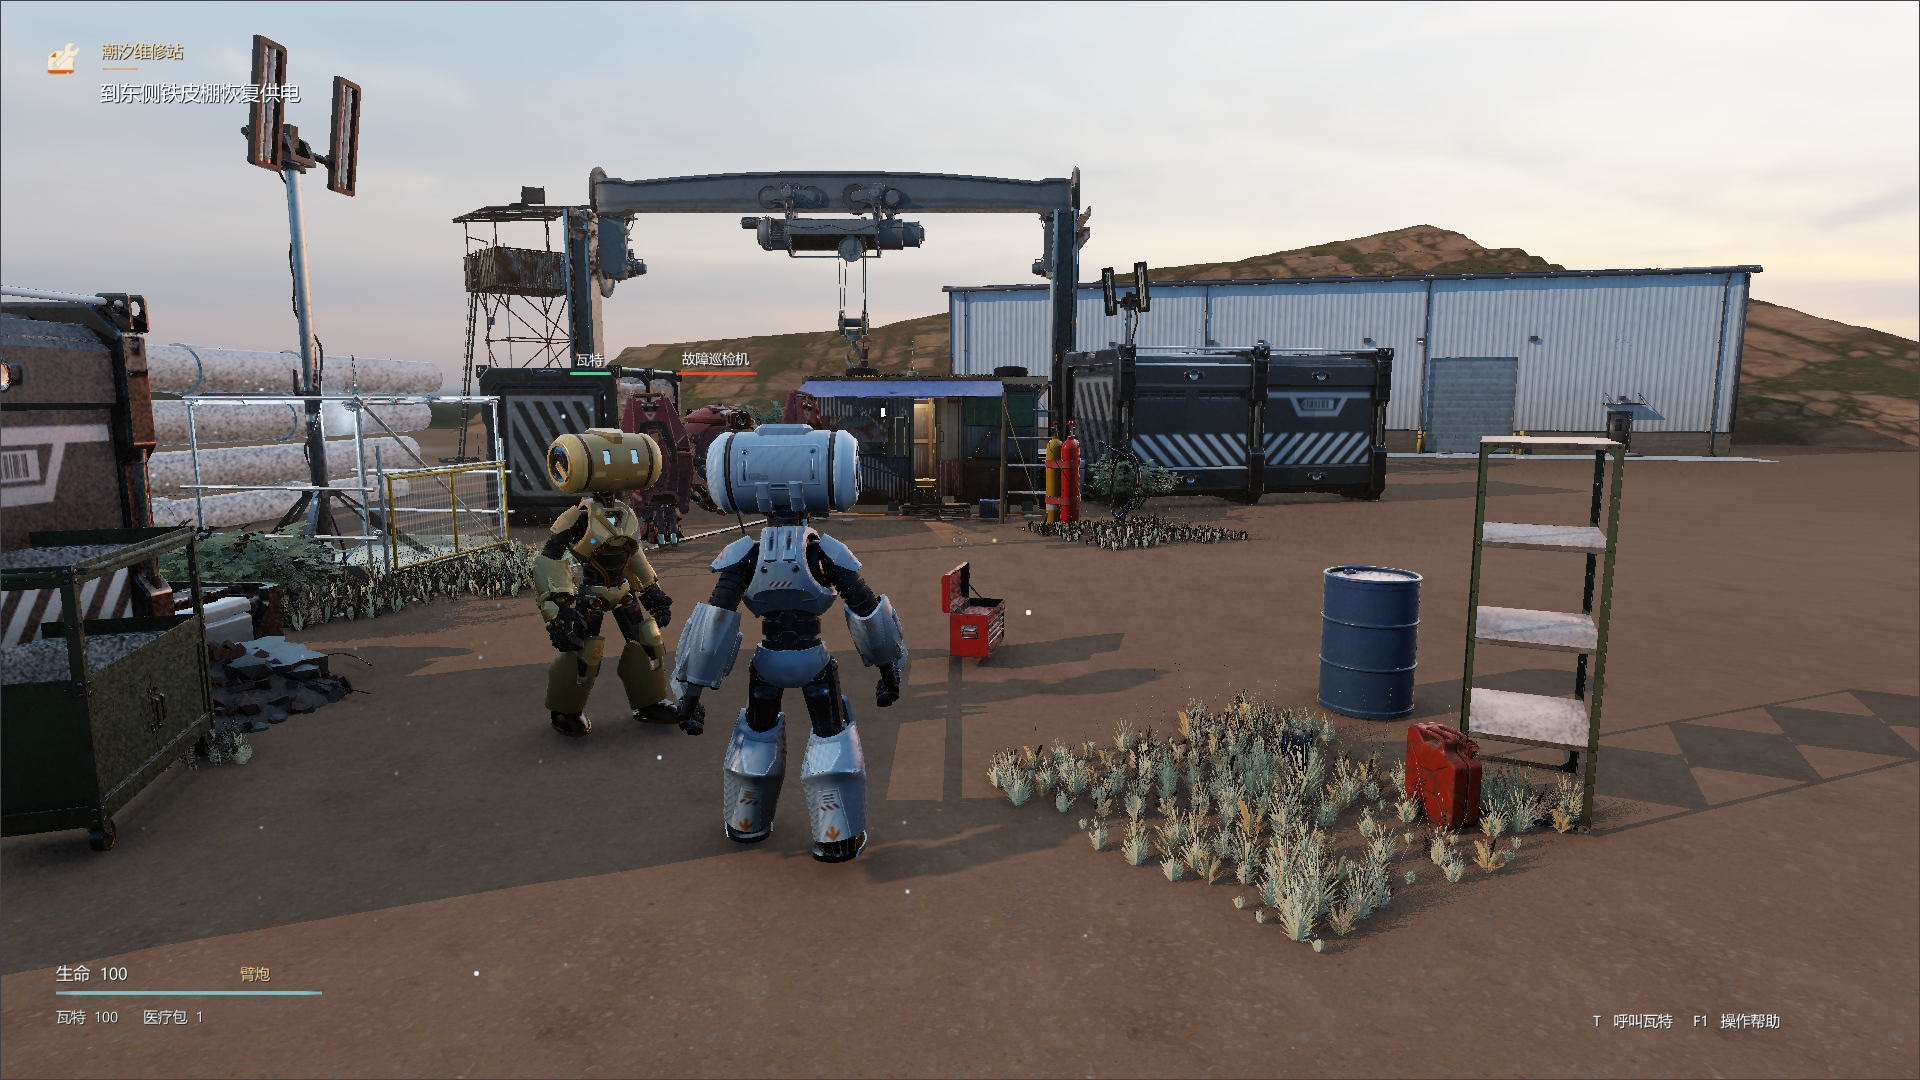
\includegraphics[width=\linewidth]{../../../output/validation/station-materials/spawn-original.png}}{原来的地面。看油桶与主角之间的空地。}
\hfill
\panelimage{.48\linewidth}{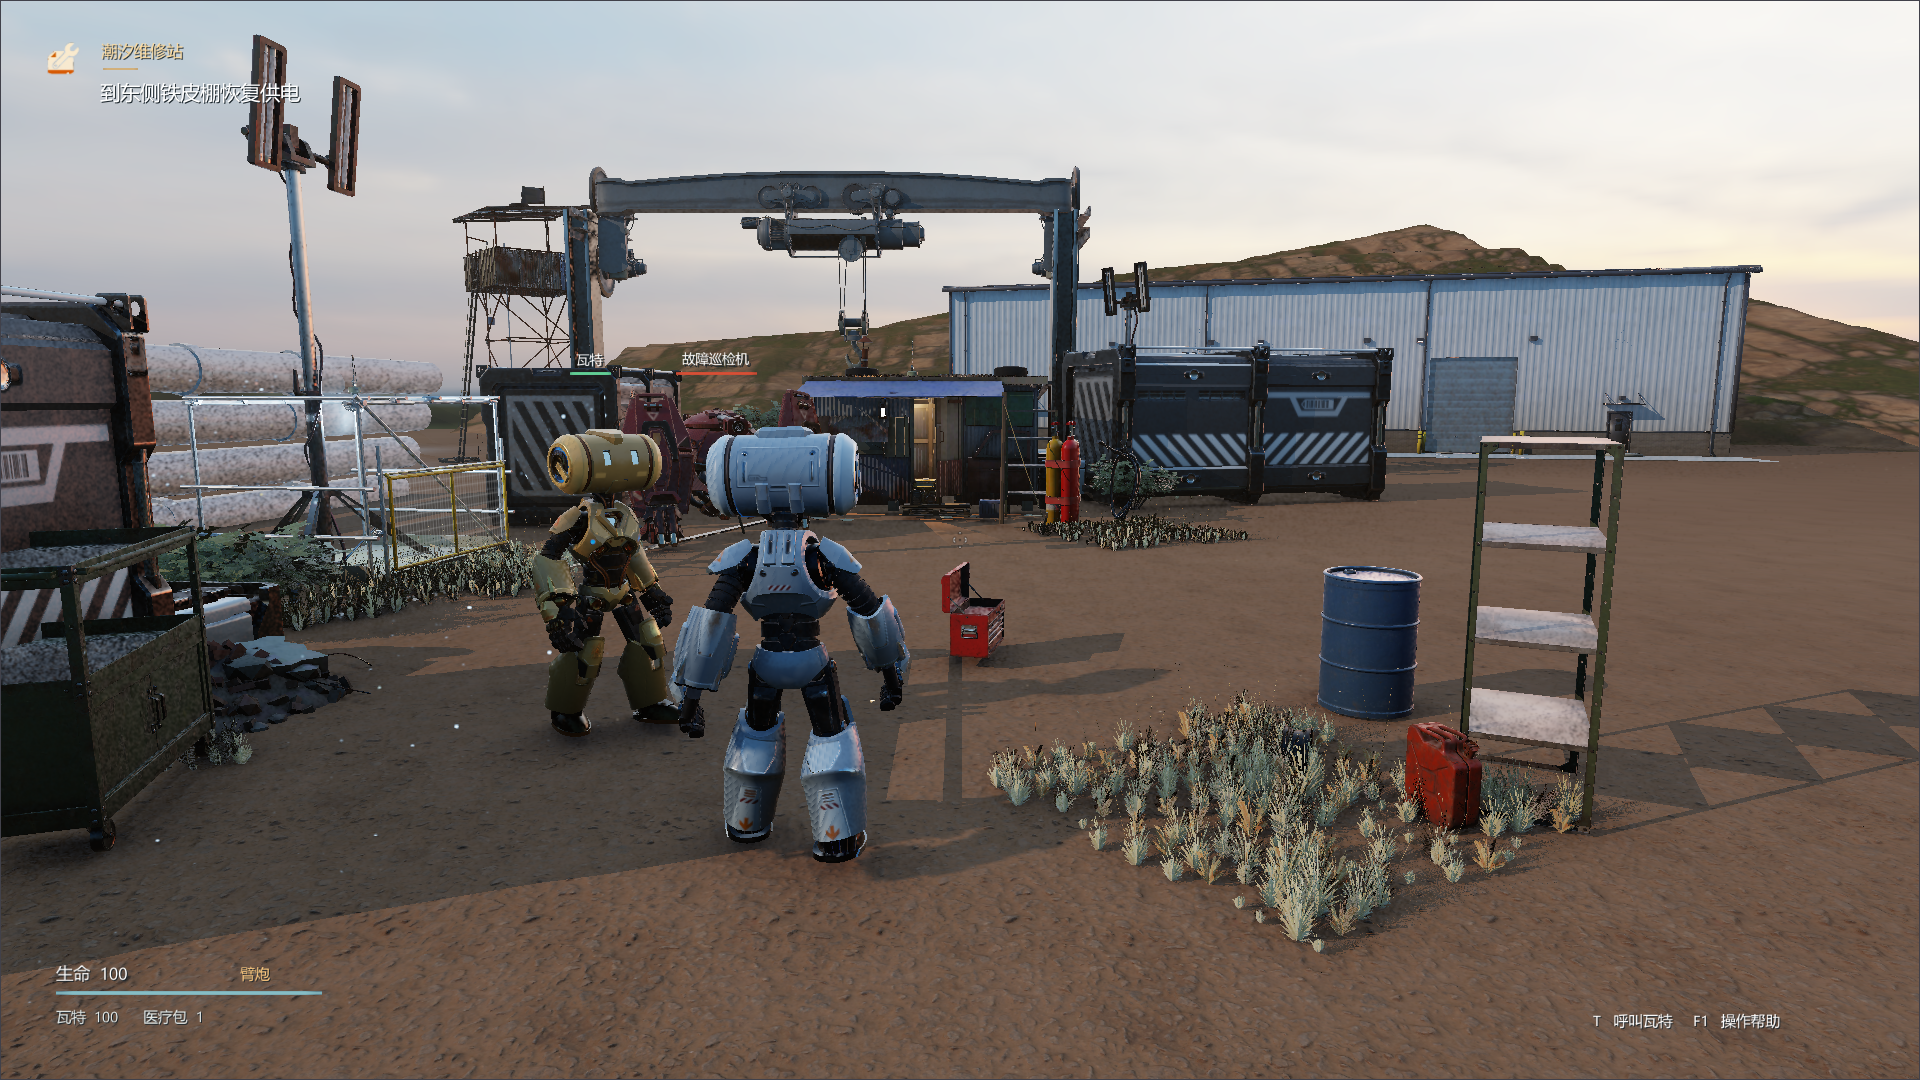
\includegraphics[width=\linewidth]{../../../output/validation/station-materials/spawn-current.png}}{修正地面缩放并启用视差，仍使用原来的日照。}
\end{center}

源网格只有一米宽。场景把沿地面的两根轴放大 100 倍，垂直轴保持原值。顶点都在平面内，因此它的位置看似正确。法线却跟着模型的逆转置矩阵变换。设原来有一条局部法线是 $(0.6,0,0.8)$，沿着地面的分量变成 $0.6/100$，向上的分量还是 $0.8$。最后把它归一化，这颗石头的斜面就几乎朝着正上方了。将三个方向都放大 100 倍，归一化后方向可以保持原样。地面四个角以及物理碰撞的位置都和原来相同。只改这一项，出生点共同可见的砂石像素中，法线改变的角度中位数为 $5.21^\circ$，底色完全一致。

接下来沿用作者扫描的颜色、法线与粗糙度，用同次扫描的灰度图改变斜看时的采样位置。示例选择 2.5 厘米的最大高差。这个网格在场景中放大了 100 倍，属性面板的“黑白高度差（模型米）”因而填 $0.025/100=0.00025$。石面的朝向继续读作者的法线图。如果对同一处起伏再从高度图算一次坡度，石头背光的一面就会被重复压暗。

\begin{center}
\panelimage{.91\linewidth}{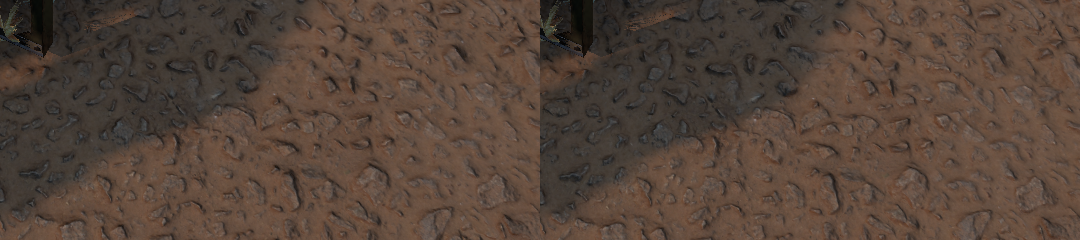
\includegraphics[width=\linewidth]{../../../output/validation/station-materials/gravel-normal-current-crop.png}}{角色走近路肩后的同一块地。左边使用作者法线，右边另开视差遮蔽。两边都从对应的 1080p 游戏原图裁取，没有重绘。}
\end{center}

\noindent 出生点写入这块地面底色和法线的 GPU 绘制，关闭视差时中位数 69.44 微秒，开启后 141.25 微秒；靠近路肩时为 126.18 和 223.33 微秒。地面每次仍只绘制两个三角形，增加的工作发生在覆盖的像素上。\readings{\refitem{https://polyhaven.com/a/gravel_road}{Amal Kumar，Poly Haven Gravel Road，CC0}；\refitem{https://learnopengl.com/Advanced-Lighting/Parallax-Mapping}{LearnOpenGL，视差遮蔽}。}

\clearpage
\subsection{工具台的漆面与备用轮毂}
靠近工具台，层板和框架几乎填满视口。原模型的底色和法线各为 1K。这里取作者发布的 4K 原片，以 2K 烘入这个工具台，同模型的另一件器材架继续使用原图。两幅游戏图中约 24.4 万个像素都看得到架子，其中约 15.8 万个像素的线性底色变化超过 0.002。

\begin{center}
\panelimage{.45\linewidth}{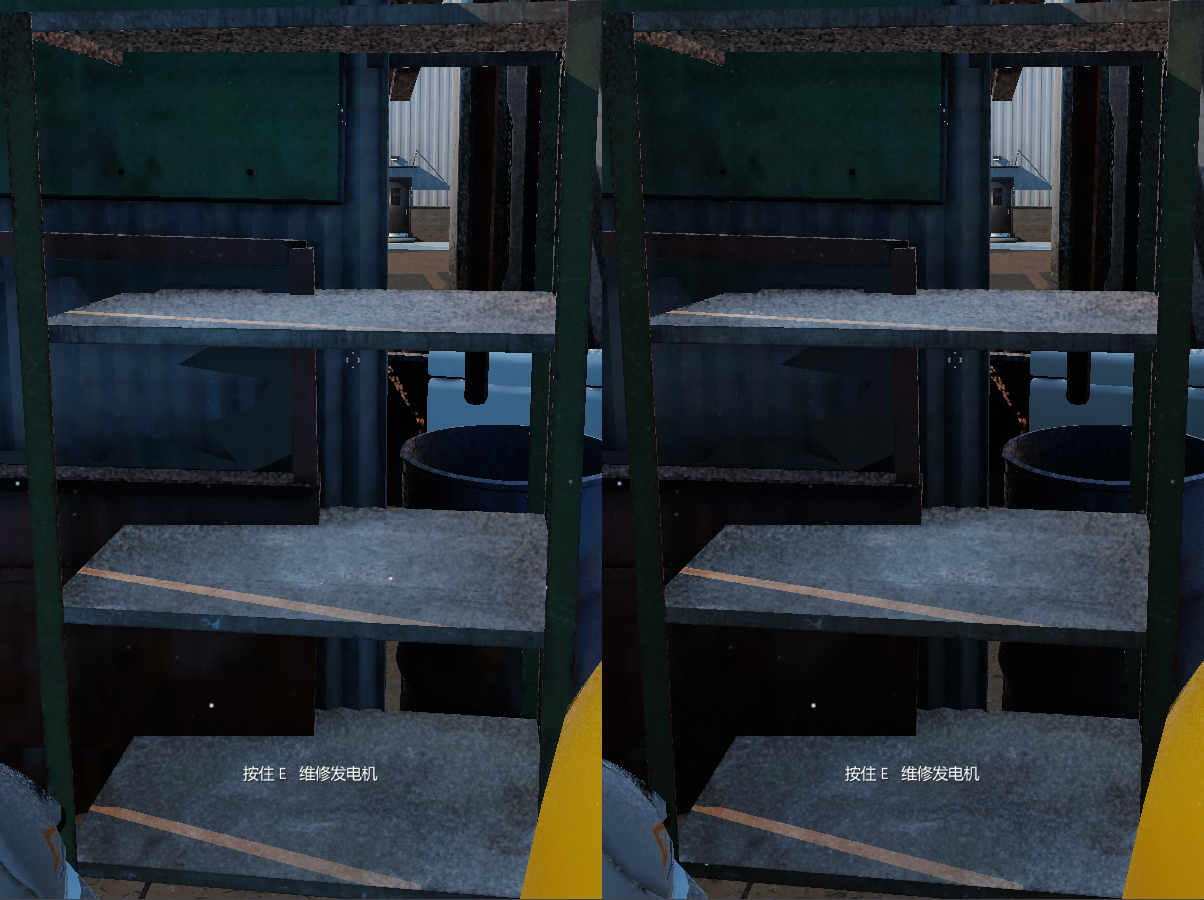
\includegraphics[width=\linewidth]{../../../output/validation/station-materials/rack-original-current-crop.png}}{工具台。左为原版，右为新图。}
\hfill
\panelimage{.49\linewidth}{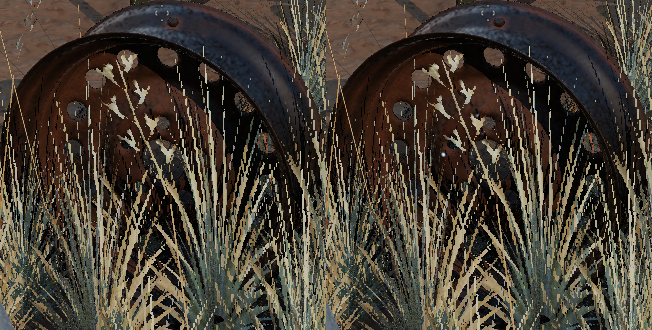
\includegraphics[width=\linewidth]{../../../output/validation/station-materials/rim-original-current-crop.png}}{备用轮毂。位移很小，须对齐外缘观察。}
\end{center}

备用轮毂直径约 40 厘米，作者的扫描网格已经保留轮孔和翻边。高度图最暗为 125，最亮为 145，中位数为 133（满白为 255）。若把白色设为原面，几乎所有顶点都会往里移。此处把“原表面的灰度”设为 $133/255\approx0.522$。顶点沿法线的位移成为 $H(g-g_0)$，其中 $g_0$ 是原面灰度。取 $H=0.025$ 米时，纹理中最高与最低两点的差为 $0.025(145-125)/255\approx1.96$ 毫米。这个数是本关卡选择的磨损深度，并非作者测量的锈层厚度。

显卡回放可以读到顶点着色后的实际位置。以近景的 49,320 个索引位置计，中位数移动 0.052 毫米，最远 0.821 毫米。投到屏幕上分别只有 0.035 和 0.511 个像素。把效果限定到玩家可以走近的这一只轮毂，就能保留这种细微变化。角色、交互和碰撞仍按关卡原有的几何工作。

工具台两份帧按旧、新、新、旧交替回放，每轮先预热再采五次。工具台绘制分别为 49.23 和 49.02 微秒（中位数），同机位两份帧中最慢的命令都是后面的计算着色。另一个机位中，轮毂关闭和开启置换绘制分别为 22.88 和 23.94 微秒，波动区间重叠。两张新增的 2K RGBA8 贴图加上完整 mip 层合计约 42.67 MiB 纹素，另一架用的旧图仍保留。这是格式计算值；实际显存驻留情况需要单独测量。

\readings{\refitem{https://polyhaven.com/a/worn_metal_rack}{Poly Haven，Worn Metal Rack}；
\refitem{https://polyhaven.com/a/rusted_wheel_rim_01}{Poly Haven，Rusted Wheel Rim 01}。实机图、四种机位、回放原始样本见 \path{output/validation/station-materials/}。}

\clearpage
\subsection{碎石上的车辙}
角色脚下的石块已有法线和视差遮蔽。从游戏的跟随相机看过去，缝隙只能说明单颗石头的起伏；同一片碎石一直铺到维修棚，路上看不出车辆经过的方向。我们沿弯道各铺一条宽约 34 厘米的胎印，轮心间距 1.54 米。泥土的颜色、法线与粗糙度取自同一块两米多宽的实物扫描。槽边露出的石头继续显示原砂石的材质，行走高度沿用原来的碰撞面。

\begin{center}
\panelimage{.48\linewidth}{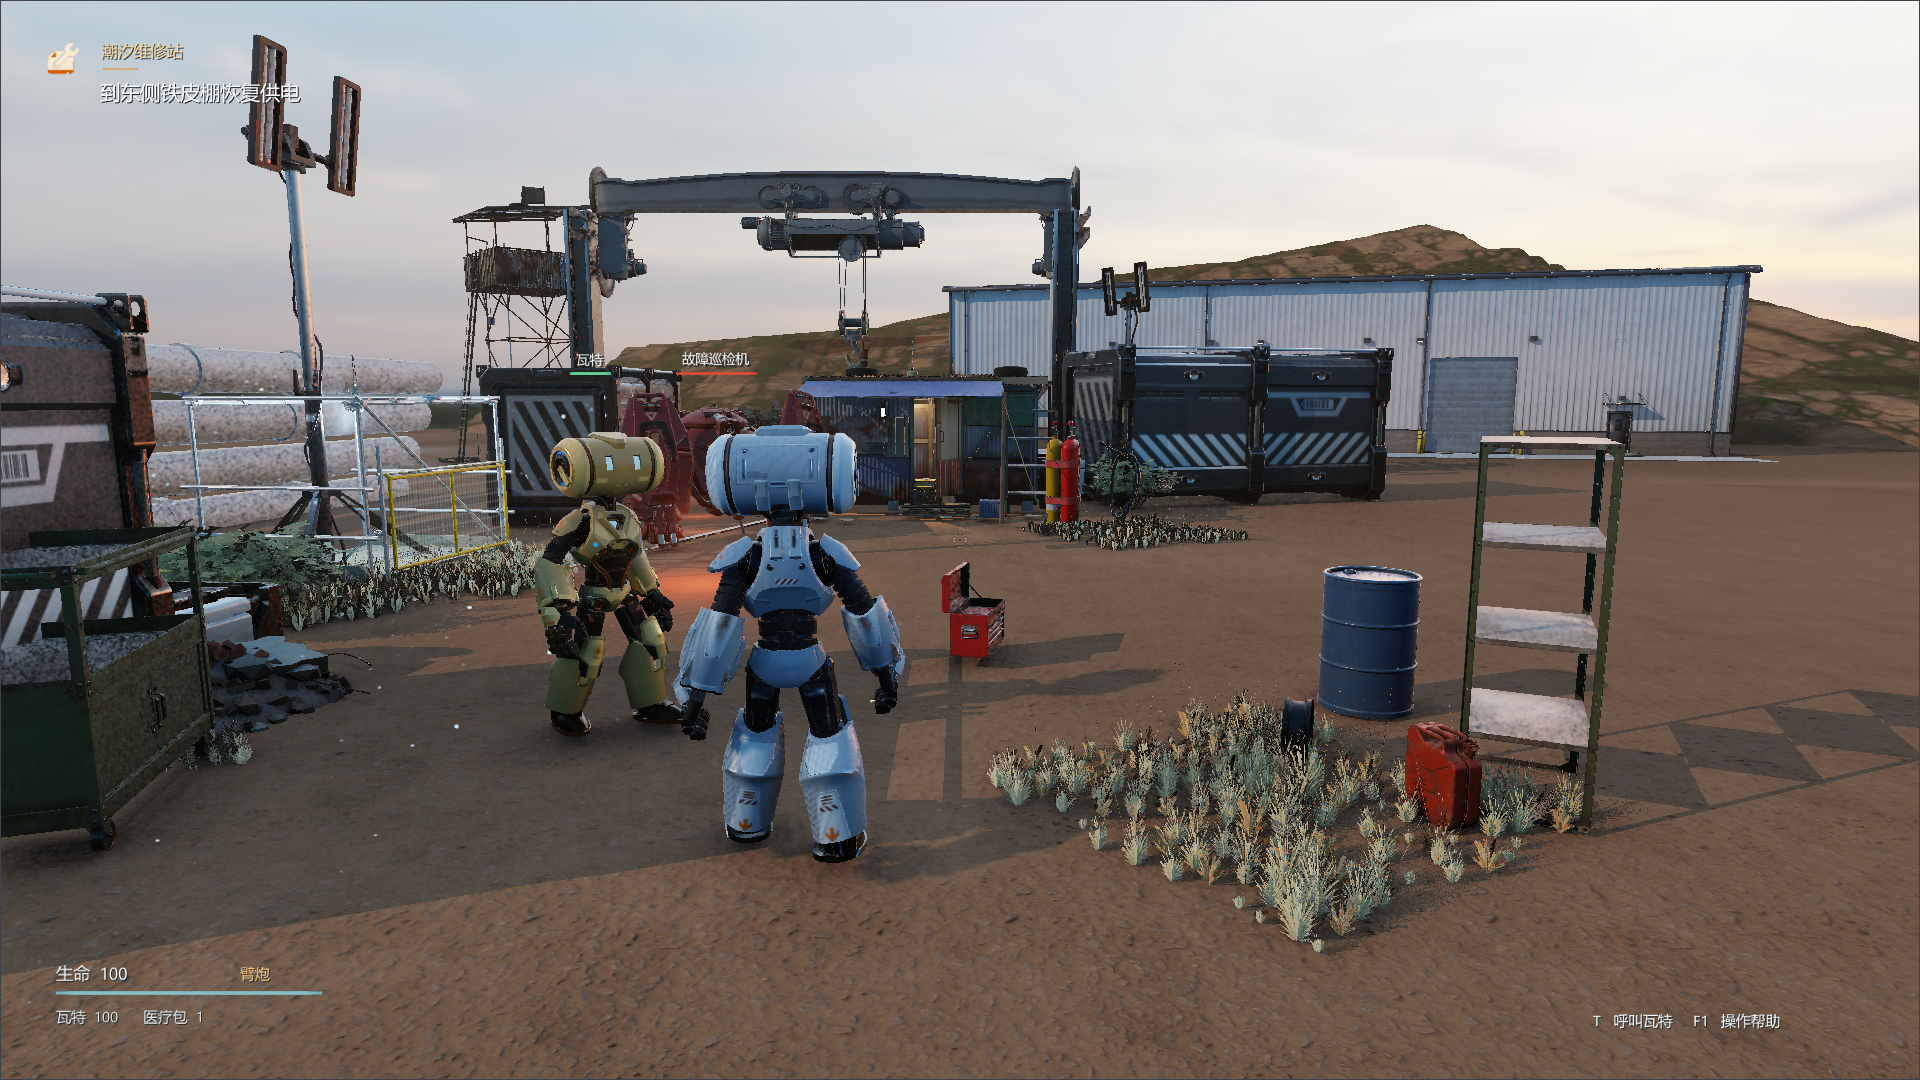
\includegraphics[width=\linewidth]{../../../output/validation/station-tracks/tracks-original.png}}{原来的视差碎石。两张都是游戏默认出生点。}
\hfill
\panelimage{.48\linewidth}{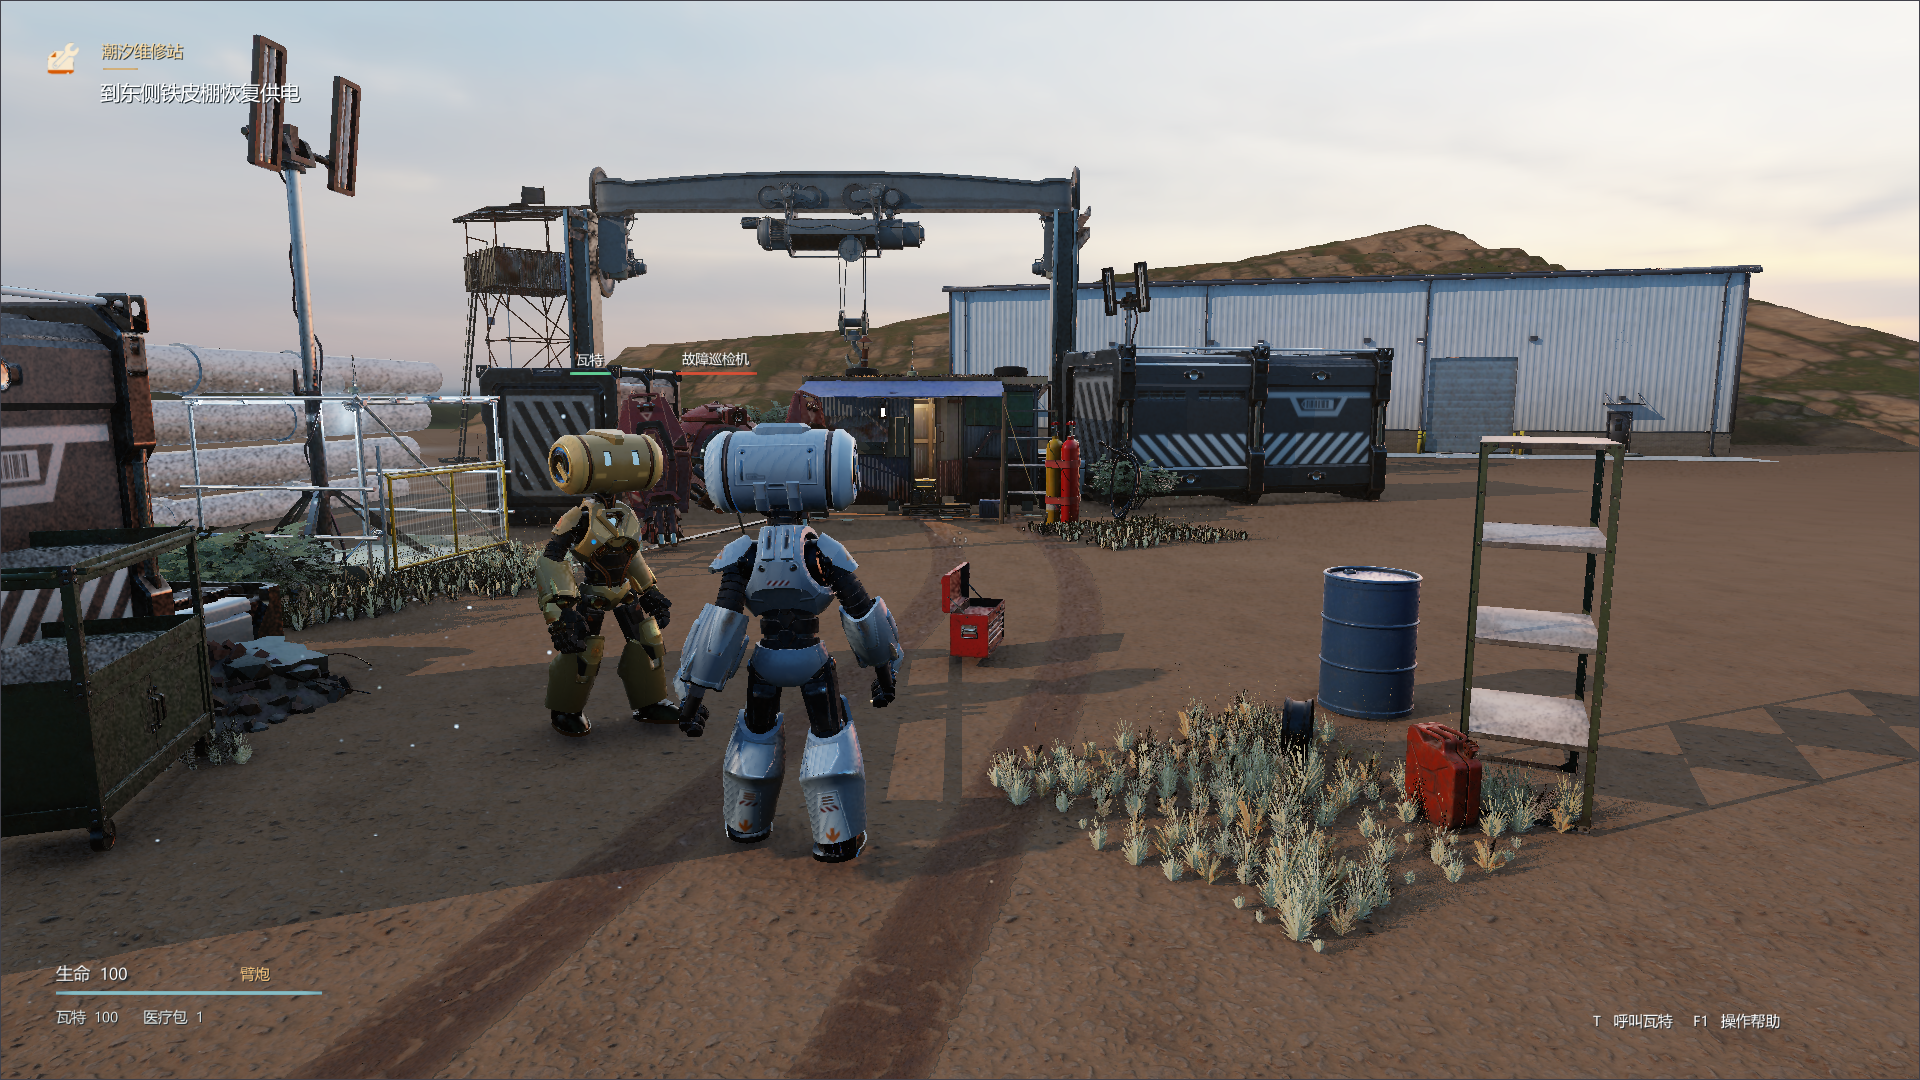
\includegraphics[width=\linewidth]{../../../output/validation/station-tracks/tracks-current.png}}{两道胎印之间仍可看到碎石，向前延伸到维修棚。}
\end{center}

同机位旧碎石覆盖 860,798 个像素，其中 86,064 个在新图中显示胎印，约占十分之一。只取这块共同可见区域，显示颜色的平均绝对差为 21.51 个 8-bit 色阶。两个模型的区分来自各次绘制前后的实际深度，可以排除角色动作对统计的影响。

地表带由九个路径点确定。正式路线分成 16 段，两道胎印合计 64 个三角形。开启后 draw 从 413 增至 415，dispatch 仍为 16 次。使用 RTX 5070 Ti Laptop GPU，在 1080p 游戏第 12 帧交替回放有无车辙的两个版本，每次预热后读五次时间，每种配置共十次。写入车辙底色和法线的那次绘制中位数为 14.58 微秒。帧内全部绘制与计算命令的时间之和，中位数从 47.17 到 44.81 毫秒，但两组 P10 到 P90 区间分别为 43.42--50.37 和 44.03--50.61 毫秒，本次没有测出整帧速度的稳定变化。CPU 提交时间未单独测量。

其他场景可用同一份地表带工具，替换路线、带宽、贴图及每次重复的米数。Forge 将它生成普通 glTF，模型和材质继续沿用既有渲染接口。\readings{\refitem{https://polyhaven.com/a/muddy_tracks}{Amal Kumar，Poly Haven Muddy Tracks，CC0}。回放帧路径、完整对照、指标和复测命令见 \path{output/validation/station-tracks/}。}
